\section{Control History and Pontryagin's Minimum Principle}

\subsection{Control History}

% 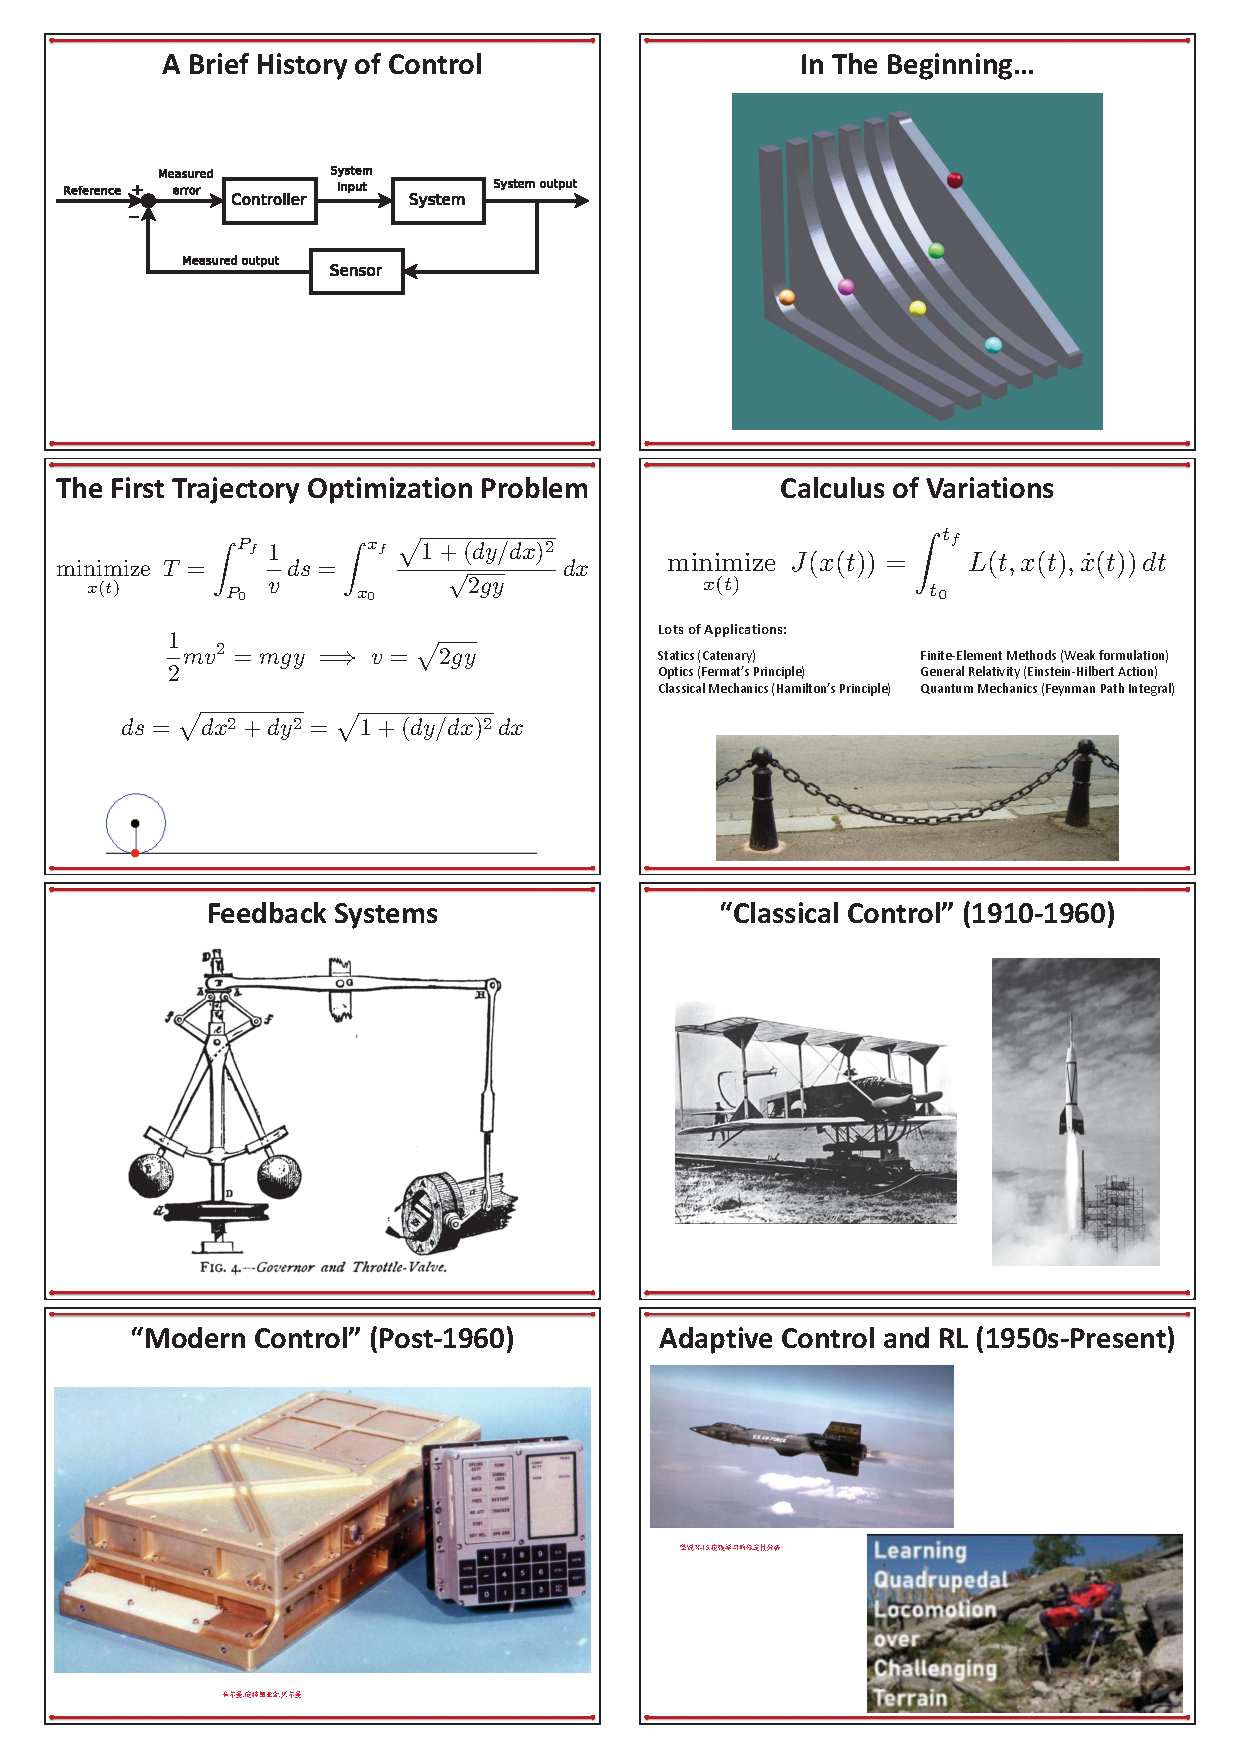
\includepdf[pages=1-,offset=0cm 0.5cm]{tex/ch6/Control History.pdf}


\begin{center}
    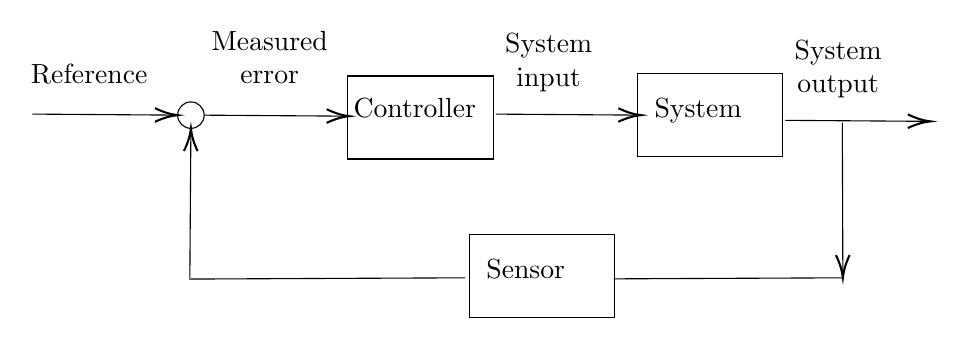
\begin{tikzpicture}[x=0.75pt,y=0.75pt,yscale=-1,xscale=1]
    \draw    (61.04,121.37) -- (129,121.86) ;
    \draw [shift={(131,121.88)}, rotate = 180.41] [color={rgb, 255:red, 0; green, 0; blue, 0 }  ][line width=0.75]    (10.93,-3.29) .. controls (6.95,-1.4) and (3.31,-0.3) .. (0,0) .. controls (3.31,0.3) and (6.95,1.4) .. (10.93,3.29)   ;
    \draw   (131,121.88) .. controls (131,118.35) and (133.85,115.5) .. (137.38,115.5) .. controls (140.9,115.5) and (143.75,118.35) .. (143.75,121.88) .. controls (143.75,125.4) and (140.9,128.25) .. (137.38,128.25) .. controls (133.85,128.25) and (131,125.4) .. (131,121.88) -- cycle ;
    \draw    (143.75,121.88) -- (211.71,122.36) ;
    \draw [shift={(213.71,122.38)}, rotate = 180.41] [color={rgb, 255:red, 0; green, 0; blue, 0 }  ][line width=0.75]    (10.93,-3.29) .. controls (6.95,-1.4) and (3.31,-0.3) .. (0,0) .. controls (3.31,0.3) and (6.95,1.4) .. (10.93,3.29)   ;
    \draw   (213,103) -- (283,103) -- (283,143) -- (213,143) -- cycle ;
    \draw    (284.25,121.38) -- (352.21,121.86) ;
    \draw [shift={(354.21,121.88)}, rotate = 180.41] [color={rgb, 255:red, 0; green, 0; blue, 0 }  ][line width=0.75]    (10.93,-3.29) .. controls (6.95,-1.4) and (3.31,-0.3) .. (0,0) .. controls (3.31,0.3) and (6.95,1.4) .. (10.93,3.29)   ;
    \draw   (352.5,102) -- (422.5,102) -- (422.5,142) -- (352.5,142) -- cycle ;
    \draw    (423.75,124.38) -- (491.71,124.86) ;
    \draw [shift={(493.71,124.88)}, rotate = 180.41] [color={rgb, 255:red, 0; green, 0; blue, 0 }  ][line width=0.75]    (10.93,-3.29) .. controls (6.95,-1.4) and (3.31,-0.3) .. (0,0) .. controls (3.31,0.3) and (6.95,1.4) .. (10.93,3.29)   ;
    \draw   (271.5,179.5) -- (341.5,179.5) -- (341.5,219.5) -- (271.5,219.5) -- cycle ;
    \draw    (451.5,200.25) -- (341.04,200.75) ;
    \draw    (269.5,200.25) -- (136.52,200.85) ;
    \draw    (136.87,200.5) -- (137.36,130.25) ;
    \draw [shift={(137.38,128.25)}, rotate = 90.4] [color={rgb, 255:red, 0; green, 0; blue, 0 }  ][line width=0.75]    (10.93,-3.29) .. controls (6.95,-1.4) and (3.31,-0.3) .. (0,0) .. controls (3.31,0.3) and (6.95,1.4) .. (10.93,3.29)   ;
    \draw    (451.23,125.5) -- (451.48,198.25) ;
    \draw [shift={(451.49,200.25)}, rotate = 269.8] [color={rgb, 255:red, 0; green, 0; blue, 0 }  ][line width=0.75]    (10.93,-3.29) .. controls (6.95,-1.4) and (3.31,-0.3) .. (0,0) .. controls (3.31,0.3) and (6.95,1.4) .. (10.93,3.29)   ;
    \draw (59,96) node [anchor=north west][inner sep=0.75pt]   [align=left] {Reference};
    \draw (142,80) node [anchor=north west][inner sep=0.75pt]   [align=left] {\begin{minipage}[lt]{48.08pt}\setlength\topsep{0pt}
    \begin{center}
    Measured\\error
    \end{center}
    \end{minipage}};
    \draw (214.5,112.5) node [anchor=north west][inner sep=0.75pt]   [align=left] {Controller};
    \draw (359.5,112.5) node [anchor=north west][inner sep=0.75pt]   [align=left] {System};
    \draw (284,81.5) node [anchor=north west][inner sep=0.75pt]   [align=left] {\begin{minipage}[lt]{36.73pt}\setlength\topsep{0pt}
    \begin{center}
    System\\input
    \end{center}
    \end{minipage}};
    \draw (423.5,84.5) node [anchor=north west][inner sep=0.75pt]   [align=left] {\begin{minipage}[lt]{36.73pt}\setlength\topsep{0pt}
    \begin{center}
    System\\output
    \end{center}
    \end{minipage}};
    \draw (278.5,190) node [anchor=north west][inner sep=0.75pt]   [align=left] {Sensor};
    \end{tikzpicture}
\end{center}

In the beginning, there was the Brachistochrone Problem, The brachistochrone problem asks for the shape of the curve down which a bead, starting from rest and accelerated by gravity, will slide (without friction) from one point to another in the least time.
\begin{figure}[H]
    \centering
    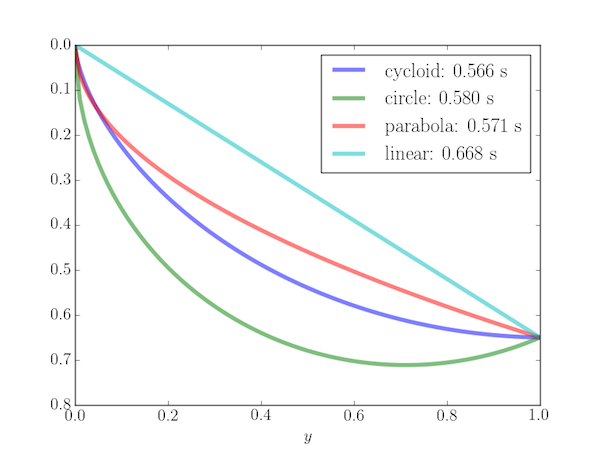
\includegraphics[scale=.5]{./tex/ch6/brachistochrone.png}
\end{figure}

\subsection{Deterministic Optimal Control}

The term ``deterministic'' is different from parameter uncertainty.

\begin{itemize}
    \item Continuous time optimal control:

    \begin{tikzpicture}[x=0.75pt,y=0.75pt,yscale=-1,xscale=1]
    %Curve Lines [id:da981836703481654] 
    \draw    (199,70) .. controls (156.82,86.2) and (132,105.81) .. (176.14,118.81) ;
    \draw [shift={(177.5,119.2)}, rotate = 195.78] [color={rgb, 255:red, 0; green, 0; blue, 0 }  ][line width=0.75]    (10.93,-3.29) .. controls (6.95,-1.4) and (3.31,-0.3) .. (0,0) .. controls (3.31,0.3) and (6.95,1.4) .. (10.93,3.29)   ;

    \draw (178,49.4) node [anchor=north west][inner sep=0.75pt]    {$\min_{\substack{x(t)\\u(t)}} J( x( t) ,u( t)) =\int _{t_{0}}^{t_{f}} l( x( t) ,u( t)) dt+l_{F}( x( t_{f}))$};
    \draw (86,125) node [anchor=north west][inner sep=0.75pt]   [align=left] {state and input trajectories};
    \draw (230,70) node [anchor=north west][inner sep=0.75pt]   [align=left] {cost function};
    \draw (303,30) node [anchor=north west][inner sep=0.75pt]   [align=left] {stage / (one) step cost};
    \draw (430,70) node [anchor=north west][inner sep=0.75pt]   [align=left] {terminal cost};
    \end{tikzpicture}

    subject to ``dynamic constraints'': $\dot x(t)=f(x(t),u(t))$. There can be more other constraints.

    \item Since the time is ``continuous'', this is an ``infinite dimensional'' problem (``infinite'' means infinite samples in continuous time):
    \begin{equation}
        u_{1:N}=\left[ \begin{array}{c}
            u_1\\
            u_2\\
            \vdots\\
            u_N\\
        \end{array} \right] ,u\left( t \right) =\lim_{N\rightarrow \infty}u_{1:N}
    \end{equation}

    \item Solutions are open-loop trajectories, there is no feedback. If there isn't any noise, it's deterministic and the same every time. In the stochastic optimal control problem because it's stochastic, open loop trajectories don't work every time anymore. So in in the stochastic setting, the solutions are feedback policies, and that's got hooks into the way people think about RL.
    \item There are a handful of toy-problems with analytic solutions but not many (especially for nasty, nonlinear problems).
    \item We will focus on the discrete-time setting which leads to tractable algorithms. Discrete time optimal control:
    \begin{equation}
        \begin{aligned}
            \min _{\substack{x_{1:N}\\u_{1:N}}}J\left( x_{1:N},u_{1:N} \right) =\sum_{k=1}^{N-1}{\left[l\left( x_k,u_k \right)\right]}+l_F\left( x_N \right)\\
            \text{s.t.}\ x_{k+1}=f\left( x_k,u_k \right)\\
            u_{\min}\le u_k\le u_{\max}\ \left( \text{torque\ }\text{limits} \right)\\
            c\left( x_k \right) \le 0\ \left( \text{Obstacle/safety\ constraint\ etc}. \right)\\
        \end{aligned}
    \end{equation}
    \item Discrete-time problem is a finite dimensional problem.
    \item Samples $x_k,u_k$ are often called ``knot point''. (I think that term comes from splines which are often used in discretize trajectories but it's a super common term)
    \item We've already introduce several method to convert continuous to discrete time using integration, i.e. Rouge-Kutta. And discrete to continuous using interpolation.
    \item Most robotic systems are pretty deterministic, there's difference between stochasticity / non-deterministic and being uncertain, when we talk about robots there's usually uncertainty in the model parameters or unmodeled things or whatever but if you run the same experiment twice you're going to get the same answer.
    \item A weird philosophical territory that weather there exist real stochastic. 
\end{itemize}

\subsection{Pontryagin's Minimum Principle}

\begin{itemize}
    \item Also called ``maximum principle'' if you maximize a reward.
    \item It is the first-order necessary conditions for deterministic optimal control problem.
    \item In discrete time, it is just the special case of KKT conditions.
    \item Given:
    \begin{equation}
        \begin{aligned}
            \min _{\substack{x_{1:N}\\u_{1:N}}}J\left( x_{1:N},u_{1:N} \right) =\sum_{k=1}^{N-1}{\left[l\left( x_k,u_k \right)\right]}+l_F\left( x_N \right)\\
            \text{s.t.}\ x_{k+1}=f\left( x_k,u_k \right)
        \end{aligned}
    \end{equation}
    We can form the Lagrangian:
    \begin{equation}
        L = \sum_{k=1}^{N-1}{\left[l\left( x_k,u_k \right) + \lambda_{k+1}^T\left(f(x_k,u_k)-x_{k+1}\right)\right]}+l_F\left( x_N \right)
    \end{equation}
    \item To make things easier, we introduce ``Hamiltonian'' (with some deep connections to classical physics): $H(x,u,\lambda)=l(x,u)+\lambda^Tf(x,u)$. By plugging $H$ into $L$ and \textcolor{red}{re-index} the stuff inside the sum, we get
    \begin{equation}
        L = H(x_1,u_1,\lambda_2) + \sum_{\textcolor{red}{k=2}}^{N-1}{\left[H(x_k,u_k,\lambda_{k+1}) - \lambda_{k}^Tx_k\right]}+l_F\left( x_N \right) \textcolor{red}{- \lambda_N^Tx_N}
    \end{equation}
    \item Take derivatives w.r.t. $x$ and $\lambda$ (KKT conditions):
    \begin{equation}
        \begin{aligned}
            \frac{\partial L}{\partial \lambda _{k+1}}=\frac{\partial H}{\partial \lambda _{k+1}}-x_{k+1}=f\left( x_k,u_k \right) -x_{k+1}=0\\
            \frac{\partial L}{\partial x_k}=\frac{\partial H}{\partial x_k}-\lambda _{k}^{T}=\frac{\partial l}{\partial x_k}+\lambda _{k+1}^{T}\frac{\partial f}{\partial x_k}-\lambda _{k}^{T}=0\\
            \frac{\partial L}{\partial x_N}=\frac{\partial l_F}{\partial x_N}-\lambda _{N}^{T}
        \end{aligned}
    \end{equation}
    \item For $u$ we write the $\min$ explicitly to handle torque limits (if $u$ is unconstraint, we can just write $\partial L / \partial u$):
    \begin{equation}
        \begin{aligned}
            u_k=\text{arg}\min _{\tilde{u}}H\left( x_k,\tilde{u},\lambda _{k+1} \right)\\
            \text{s.t.\ }\tilde{u}\in \mathcal{U}\ \left( \text{short hand for ``in feasible set''} \right)\\
            \text{e.g.}\  u_{\min}\le \tilde{u}\le u_{\max}
        \end{aligned}
    \end{equation}
    The relationship between these stuff and Hamiltonian mechanics is: the first two lines are Hamilton's equations and lambda is the momentum. The top line is literally just the Dynamics like we already did, it goes forward in time, it's $x_k$ plug-in, you can get $x_{k+1}$. The second line is some other equations, look at the $\lambda$, I got $\lambda_k$ on the left and I got $\lambda_{k+1}$ on the right, that one goes backwards in time. So this sets us up for some interesting stuff: $x_k$ stuff goes forward in time and the $\lambda_k$ stuff goes backward in time and we get boundary conditions $x_0$ on start time, $\lambda_N$ on final time based on the terminal cost. This is where the shooting method's idea coming from, shoot forward with dynamics and backward with lambdas and somehow get these to match up in the middle.

    \begin{enumerate}
        \item we get $x_0,\lambda_N$, initialize $u$ trajectory.
        \item forward rollout to get $x_1, \cdots, x_N$
        \item now we have $x,u$, backward iteration to get $\lambda$.
        \item now we have $x,u, \lambda$, solve the constraint optimization problem to get $\Delta u$, use line search method. Back to step 2.
    \end{enumerate}
    无论系统本身是线性的还是非线性的（线性的系统局部线性化就等于本身），我们一直分析的是类似$\Delta\dot x=A\Delta x+B\Delta u$这种系统，迭代法寻找的总是$\Delta u$，因为一切的一切比如$\lambda,x$都是在上一个$u$的基础上获得的，我们经过rollout后得到的值。从上面这几步可以看出，基于shooting方法迭代求解该方程，需要有一次正向传播过程，再有一次反向传播过程，这就很像训练神经网络的梯度下降更新权重的过程。这个过程实际是比较慢的，下节会举例对比说明，所以在现代，基本都不会根据这个流程做了，这种方法无论是收敛性、数值优劣和鲁棒性都不够强。
    \item These can be stated almost identically in continuous time:
    \begin{equation}
        \begin{aligned}
            \dot{x}=\nabla _{\lambda}H\left( x,u,\lambda \right)\\
            \textcolor{red}{-}\dot{\lambda}=\nabla _xH\left( x,u,\lambda \right)\\
            u=\text{arg}\min _{\tilde{u}}H\left( x,\tilde{u},\lambda \right)\\
            \text{s.t.\,\,}u\in \mathcal{U}\\
            \lambda \left( t_f \right) =\frac{\partial l_F}{\partial \lambda}\\
        \end{aligned}
    \end{equation}
\end{itemize}

\subsection{Some Notes}
\begin{itemize}
    \item Historically, many algorithms were based on integrating the continuos ODEs forward/backward to do gradient descent on $u(t)$. (such as neural ODEs)
    \item These are called ``indirect'' and/or ``shooting'' methods. (awful performance)
    \item In continuous time $\lambda(t)$ is called ``co-state'' trajectory, also is the gradient of cost-to-go.
    \item These methods have largely fallen out of favor as computers have improved.
\end{itemize}